\documentclass[letterpaper, 11pt]{article} 

\usepackage{graphics,graphicx}
\usepackage{multicol} 
\usepackage{parskip}
\usepackage{amsmath}
\usepackage{multirow}
\usepackage[english]{babel}
\usepackage[utf8]{inputenc}
\usepackage{fancyhdr}
\usepackage[title]{appendix}
\usepackage{wasysym}
\usepackage{url}
\usepackage{hyperref}
\hypersetup{
    colorlinks,
    citecolor=black,
    linkcolor=blue,
    filecolor=magenta,
    urlcolor=blue,
}

\usepackage[font=footnotesize,labelfont=small]{caption}
\captionsetup{width=0.85\linewidth}

\RequirePackage{geometry}
\geometry{margin=2cm}

\selectlanguage{english}
\setlength{\parskip}{0.2cm}
\setlength{\parindent}{0pt}


%----------------------------------------------------------------------------------------
%	BASIC INFO
%----------------------------------------------------------------------------------------


\title{Report of our work on Job Shop Scheduling using D-Wave System's Quantum Annealing}
\author{
Marek Subocz, Krzysztof Kurowski \\
\textit{Poznan Supercomputing and Networking Center (PSNC)}
}
\date{10 Oct 2019}
%--------------------------------------------------------------------------------CUERPO-----------------------------------------%
\begin{document}
\maketitle
We attempted to harness Quantum Computing speed to improve the 
performance of already existing heuristics, particularily 
for Job Shop Scheduling Problem. Our main concern was to bypass
its small number of computing units, and therefore small size
of a computable instance, to acquire the advantage of quantum
mechanics in D-Wave's quantum annealing algorithm. 
\vspace{10pt}
\begin{multicols}{2}


\section{Introduction}
All of the concepts described below until \ref{subsec:toolate} are based on this paper \cite{main_paper}.
\label{sec:intro}

\subsection{Problem definition}
The JSP is a minimization problem consisting of  a set of jobs 
$J = \{\textbf{j}_1,\dots,\textbf{j}_N\}$
that must be scheduled on a set of machines
$M = \{\textbf{m}_1, \dots, \textbf{m}_M\}$. 
Each job consists of a sequence of operations that have to be performed
in a predefined order:
\begin{equation}
\textbf{j}_n = \{O_{n1} \rightarrow O_{n2} \rightarrow \dots \rightarrow O_{nLn}\}
\end{equation}
Each operation has only one machine it can be performed on and an
integer execution time $t_{nj} \geq 0$.
Also, there can only be one operation running on a given machine at 
any given point in time and each operation of a job needs to complete 
before the following one can start. The main objective is to schedule
all operations in a valid sequence while minimizing total schedule time.


\section{Quantum annealing structure}
\label{sec:QAS}
In order to pass our problem to D-Wave's quantum computer,
it is needed to formulate it as a Quadratic Unconstrained Binary
Optimization Problem (QUBO).

\subsection{QUBO Problem Formulation}
With our approach we define a given JSP instance 
with $n_O * T$ binary variables, where $n_O$ is the total number of 
operations and $T$ is the upper bound for considered scheduling times. 
Every operation has a binary variable for every point in time:
\begin{equation}
    x_{i,t} =
    \begin{cases}
        \text{ 1 : operation $O_i$ starts at time $t$,} \\
        \text{ 0 : otherwise.}
    \end{cases}
\end{equation}

\subsection{Constraints}
It would be too expensive and imprecise to perform a quantum 
annealing computation on all these variables and combinations of
possible outcomes. Because of that, we put some constraints on
what is regarded as a viable solution and eliminate (lock on the
value of 0) some of the variables completely.
\subsubsection{One start constraint}
Every operation needs to have just one start point and therefore all of
it's variables need to sum to one. 
\subsubsection{Precedence constraint}
Every operation needs to start after the previous one from the same job
has ended. We make sure of that by checking if every operation's 
start point occurs at $previous\_start\_point + previous\_length$ or later.
\subsubsection{Share machine constraint}
Every machine can perform up to one operation at a time. To assure that
this constraint is not violated, we group all of the variables by it's
corresponding machines and check if the operations interfere in any way.

\subsection{Variable pruning}
Some of the QUBO variables can be eliminated in a precomputing phase,
improving the robustness of quantum annealing. 
% TODO: graph edge cutout picture
\subsubsection{Too early for a task}
We disable all of the variables $0 \leq x_{i,j} < S$, where $S$ is the sum
of lengths of all the operations \textbf{prior to} the considered one in the same job.
\subsubsection{Too late for a task}
\label{subsec:toolate}
We disable all of the variables $T-S \leq x_{i,j} < T$, where $S$ is the sum 
of lengths of all the operations \textbf{after} the considered one in the same job.
\subsubsection{Disabled regions}
\label{disabled_regions}
By using ''disable\_till'' and ''disable\_since'' dictionaries we can turn
off any machine from start to any point in time.
\subsubsection{Other disabled variables}
\label{disabled_variables}
There is also a possibility to disable any set of variables that we want,
implemented in the code as ''disabled\_variables'' array.


\section{Heuristic's overview}
Our heuristic approach is in many ways similar to the local search algorithm,
although it's not quite the same. It's about solving small parts of the 
instance within a time window of a given, solvable length. After exploring 
and improving the schedule in the time window, it moves one unit further and
the procedure is repeated.

\subsection{Greedy algorithm}
In order to use our heuristic approach, we need to already have a solution
that we will improve. While the best type of solution combining
diversity of possible paths to take and starting 
reliably close to an optimum is a subject for debate, we used a simple
algorithm, taking first unscheduled operation of every job and putting it as
early as possible in the general schedule.

The result of this solution will also serve as an upper bound on
the length of our schedule.

\subsection{Time window}
This was probably the most challenging part to implement, becuase we needed to
cut out a portion of a schedule without compromising it's integrity and making
sure it's independent of the rest of the problem. \\
First of all, we iterate over and check if they fit in one of those three
categories, where:
\begin{itemize}
\item $t_{o_i}$ is the start time of operation i,
\item $w_{begin}$ is the start time of the window,
\item $w_{end}$ is the end time of the window
\item $s_i$ is the operation i length
\end{itemize}

\includegraphics[width=\linewidth]{window.png}
Operations filled with red color are reaching out of the time
window and therefore treated differently. Given that operations
A and B belong to the same job, operation A will not be scheduled
in time when operation B happens, even though operation B will be
removed from the schedule.

\textbf{A}: Inside the time window
\begin{equation}
    \begin{cases}
        t_{o_i} \geq w_{begin}\\
        t_{o_i} + s_i < w_{end}
    \end{cases}
\end{equation}
We include those operations in a new dictionary of jobs, creating a smaller
instance.
\smallskip

\textbf{B}: Reaching out of the window from the left side
\begin{equation}
    \begin{cases}
        t_{o_i} < w_{begin}\\
        t_{o_i} + s_i < w_{end}
    \end{cases}
\end{equation}
We turn off (section \ref{disabled_regions}) the machines when those operations 
occupied them and prevent the next operation in the same job from starting 
before this one ends with \ref{disabled_variables}
\smallskip

\textbf{C}: Reaching out of the window from the right side
\begin{equation}
        t_{o_i} + s_i \geq w_{end}
\end{equation}
Respectively to \textbf{B}, we disable proper machine when those
operations take place and prevent the previous operation in the
same job from interfering with this one.

\section{Results}
\subsection{Single-annealing method}
First of all, we implemented a Quantum Job Shop Scheduling algorithm
described in \cite{main_paper}. At the start, the code was based on
\url{https://github.com/dwavesystems/demos/tree/master/job-shop-scheduling},
but we shifted towards an implementation that is better suited for
the heuristic approach later on. 

During testing of the algorithm, we found out that the best value to
estimate the quality of an annealing process that happened is
the number of error solutions that came out of it. In other words,
the number of times that a quantum computer didn't manage to
find a solution that satisfies all of the constraints.

\subsubsection{Chain strength}
First of all, we checked what value of chain strength is the best for
Quantum JSP annealing. During this experiment, we used a set of 4 jobs,
each consisting of 4 operations, with a maximum considered scheduling
time equal to 7. It turned out that the best chain strength
value for this particular problem is around 2.0:
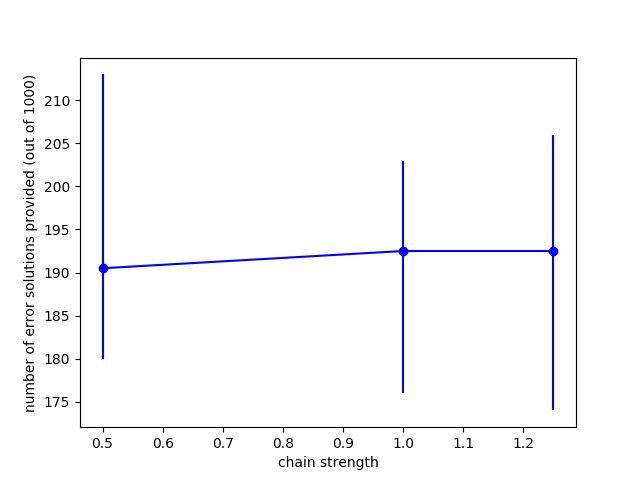
\includegraphics[width=\linewidth]{chain_strength.png}
It's important to note that the results were quite unstable and
varied from measurement to measurement, but the general conclusion
remained the same.

Also, we cannot provide any explanation why that is the case, because
the impact that chain strength has on D-Wave's machine work is largely
undiscovered. 

\subsubsection{Number of jobs}
The next experiment we did was checking which parameters are especially
important for the quality of our scheduling. First to check, how much
number of jobs affect annealing's accuracy. During this test we compared
scheduling of one job consisting of n operations with n jobs consisting of
one operation each. Each operation was 1 time unit long and was executed
on the same machine. This way we did our best to make sure no other
parameter interfered with the results: 
\includegraphics[width=\linewidth]{job_vs_operations.png}
Some of the scheduling tests with multiple jobs couldn't be run because of
an inability to pass them into the QUBO format because of too many constraints
taken into consideration. 

\subsubsection{Max time value}
Another value to consider is max\_time. It specifies the upper bound
for how long in time can a schedule be. The tests were performed
on an instance with 3 jobs, each with 3 operations, which optimal
time was equal to 4 units.
\includegraphics[width=\linewidth]{max_time.png}
Why does that graph looks like that even though, the closer
max\_time value is to an optimal total schedule time, the better? As optimal
solutions are relatively hard to find, it is harder to obtain a valid solution
when the gap between max\_time and an optimal value is really small.
Later on, when max\_time is too big, the possibilities are too vast
and the machine struggles to find any solutions.

\subsection{Partial - bruteforce method}
Final results of our algorithm were heavily reduced by the
possibilities of current quantum computers, as well as by the
specification of JSP problem, as it is exceptionally hard to
separate parts of it, while maintaining the parts big enough to
matter.

At this stage in the Quantum Computing development, the machines
are not quite reliable and error-free as we would expect from 
modern classical computers. This caused our algorithm to, in rare
occasions, receive an invalid schedule without knowing about it.
Despite some error checking, it was sometimes challenging to 
recover from such a situation.

Furthermore, in our instances we faced operations that were as
big as 10 units, even in the smallest ones. This caused the 
algorithm to consider one or two operations per job most of 
the time, so our exploring ability was substantially reduced.

\subsection{Summary}
It turned out that the limitations of currently available quantum 
computers forced us to limit the window's size to around 14 units.
This value is not big enough when we aim to find significant 
improvements in a long schedule, reaching at least 55 time units.

We look forward to improving our approach for large-instance
quantum annealing, as this a report of just a beginning of
our work.



\end{multicols}
\newpage
\begin{thebibliography}{9}

    \bibitem{main_paper} 
    Davide Venturelli, Dominic J.J. Marchand, Galo Rojo \\
    \textit{Job Shop Scheduling Solver based on Quantum Annealing} \\
    Quantum Artificial Intelligence Laboratory (QuAIL), \\ NASA Ames
    U.S.R.A. Research Institute for Advanced Computer Science (RIACS), \\
    1QB Information Technologies (1QBit),  2016\\
    \url{https://arxiv.org/pdf/1506.08479v2.pdf}

\end{thebibliography}

\end{document}

% TODO: liczba i topologia połączeń kubitów